\section{Empirical Results}
\label{sec:experiments}

In this section, we evaluate the efficacy of our graph-based conformal compression framework. Our focus is on the combinatorial optimization challenge mirroring the fixed context setting (Section~\ref{sec:fixed}): compressing a large, complex set of candidate outputs (hyperedges) into a compact subgraph.    We consider two experimental settings: a  \textit{Navigation} setting based on road networks to study the trade-off between conformal calibration and compression, and a \textit{Trip Planning} simulation designed to test the algorithm's ability to recover planted structures. We present the real-world Navigation experiment in Appendix~\ref{sec:real}.

\subsection{Navigation}
\label{sec:nav_experiments}
In this setting, hyperedges correspond to routing paths in the graph, and hypergraph vertices correspond to edges in the graph.  We compare our LP-based algorithm against {\em greedy baselines}, which select graph edges strictly order of traffic frequency (number of paths). 

We consider both the ability of the algorithm to compress a set of routes by comparing to a greedy baseline, as well as the conformal coverage $\phi$ that ensues. We study the latter in the split conformal framework of Section~\ref{sec:fixed_optimal}: We generate hyper-edge samples $\{Y_j\}_{j=1}^{T/2}$ (denoted ``training'') and $\{Y_j\}_{j=T/2+1}^{T}$ (denoted ``test'')  from the same underlying model. We use the procedure in Section~\ref{sec:fixed_optimal} to find a nested sequence of subgraphs on the training samples, and choose a subgraph as described there to obtain coverage $\phi$ on the test samples. Note that by Theorem~\ref{thm:mon}, the nested subgraph sequence is fixed and oblivious to the parameter $\kappa$ (which is only needed to state Theorem~\ref{cor:efficiency}). Further, the number of sampled routes in our experiments is small enough that the LP method runs in under a minute for our instances. 

\paragraph{Greedy Baselines.} We consider two greedy baselines. In {\sc Forward Greedy}, we sort edges in decreasing order of number of training paths they cover, and choose them in this order till a desired coverage $\phi$ is achieved on the test samples.%\footnote{Note that since this problem is more akin to densest subgraph than set cover, we cannot use marginal coverage.} 
The {\sc Reverse greedy} algorithm is a generalization of the greedy vertex deletion algorithm in~\cite{charikar2000greedy} to hypergraphs. Specialized to routing, it deletes edges in reverse order of traffic intensity (number of training paths); however, when it deletes an edge, it deletes all training paths passing through it, and recomputes traffic intensity on the left-over edges. We repeat till the coverage on the test samples falls below $\phi$, stopping just before that.  Such greedy algorithms are clearly monotone and will therefore yield conformal guarantees analogous to the LP method. However, as we show in Appendix~\ref{sec:real}, they will not provide a compression guarantee analogous to Theorem~\ref{thm:main-det}.

We will compare the number of edges used by the LP and greedy solutions for different values of  $\phi$. This allows us to study the calibration-compression trade-off  without the need to simulate a predictive model. 

%We present the synthetic experiment below, and defer the experiment on the real-world dataset to Appendix~\ref{sec:real}.


\begin{figure*}[t]
    \centering
    % --- Subfigure (a): The Selection Maps ---
    \begin{subfigure}[b]{0.22\textwidth}
        \centering
        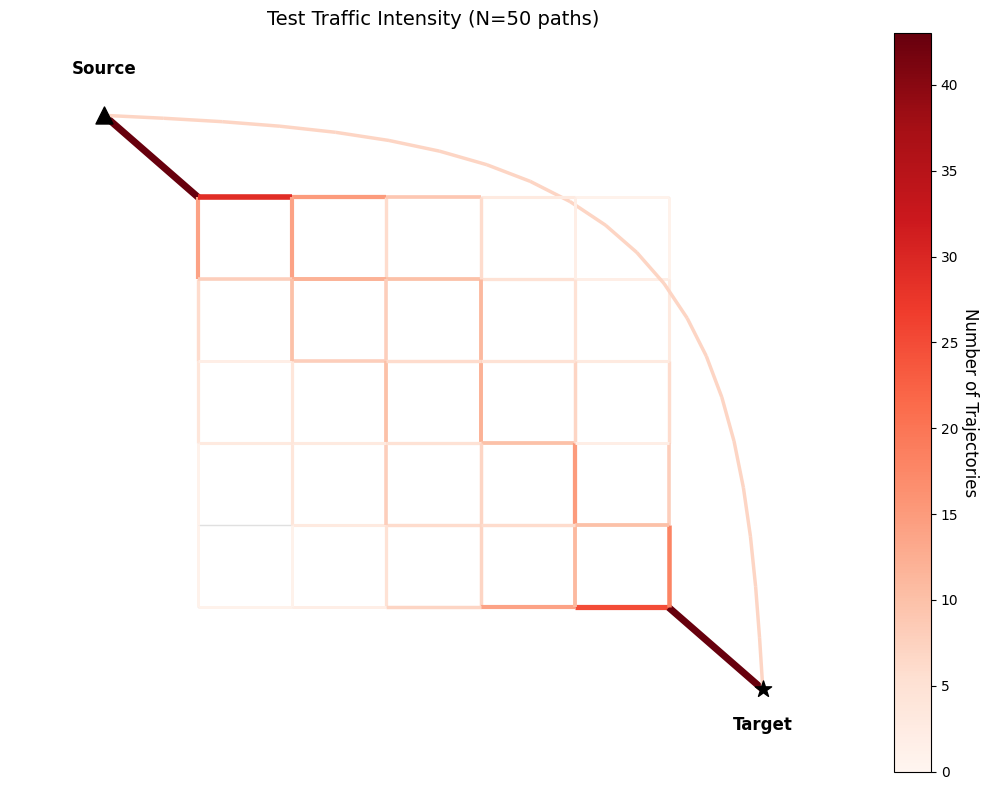
\includegraphics[width=\linewidth]{images/synthetic_heatmap2.png} 
        \caption{Traffic Heatmap.}
        \label{fig:diagonal_visual1}
    \end{subfigure}
    % --- Subfigure (b): The Curve ---
    \begin{subfigure}[b]{0.42\textwidth}
        \centering
        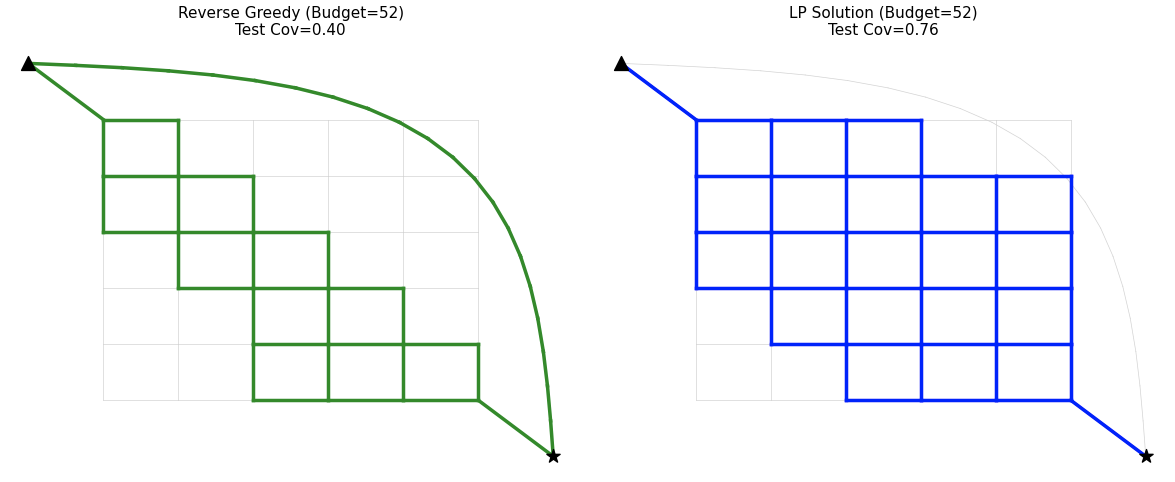
\includegraphics[width=\linewidth]{images/synthetic_reverse_map3.png}
        \caption{Reverse Greedy and LP solutions with $52$ edges.}
        \label{fig:diagonal_curve}
    \end{subfigure}
    \begin{subfigure}[b]{0.32\textwidth}
        \centering
        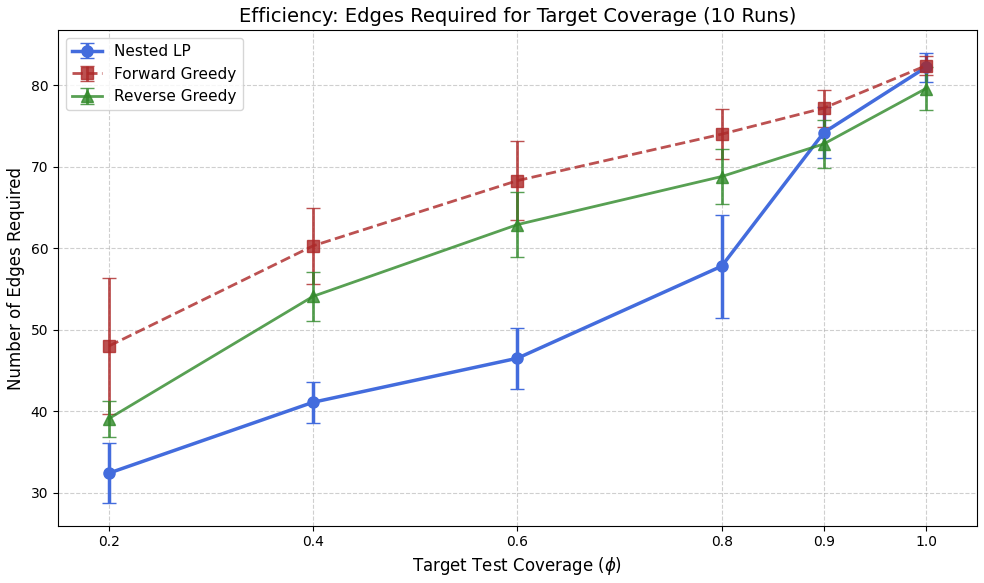
\includegraphics[width=\linewidth]{images/synthetic_reverse_eff3.png} 
        \caption{Coverage plot averaging $10$ runs.}
        \label{fig:diagonal_visual2}
    \end{subfigure}
    \caption{Analysis of the synthetic urban routing scenario. }
    \label{fig:diagonal_combined}
\end{figure*}

\paragraph{Synthetic Routing Experiment.}
This simulation tests a realistic routing scenario where traffic between two points either takes a fast, but long bypass, or takes a city grid between the two points. %Note that though our framework in Section~\ref{sec:model} can handle multiple source-sink pairs from multiple graphs in the calibration set, we experiment with this fixed context setting (Section~\ref{sec:fixed}) to highlight the calibration-compression trade-off better.
We simulate a $6 \times 6$ grid. Traffic flows from a single source at the top-left to a single target at the bottom right.  We use this grid to sample $85\%$ of the paths using shortest-paths with random edge weights, where the weight on an edge is {\tt Uniform}$[0.1,2]$. There is a bypass route from the source to the target with $20$ edges that is taken by $15\%$ of the traffic. We generate a calibration set (train) and held out (test) set of $50$ routes.   The traffic heatmap is shown in Figure~\ref{fig:diagonal_combined}(a). The paths spread out in the middle of the grid, leading to lower traffic intensity there.   

Such a setting is not only the simplest instantiation of routing, but is also quite realistic for routing in urban areas such as Manhattan, where streets can get congested unpredictably, but there are a plethora of alternate routes. 

We implement the LP and greedy calibration procedures as described above. Figure~\ref{fig:diagonal_combined}(c) shows the number of edges used by the LP and greedy solutions, where the $x$-axis shows the test coverage $\phi$.  Note that the LP solution is significantly more compressed than either greedy algorithm for all $\phi \le 0.8$.  In Figure~\ref{fig:diagonal_combined}(b), we show the edge selections when the LP solution chooses $52$ edges ($\phi = 0.75$) and the reverse greedy algorithm is made to choose the same number. The reverse greedy algorithm prioritizes the highway edges, while the LP correctly identifies that the urban center, while consisting of individually lower-frequency edges, is needed for coverage, and omits the highway entirely.



